\documentclass[]{beamer}
\usepackage[utf8]{inputenc}
\usepackage{xeCJK}
\usepackage{graphicx}
\usepackage{subfigure}
\usepackage{mathtools}
\usepackage{utopia} %font utopia imported
\usetheme{CambridgeUS}
\usecolortheme{dolphin}
\usefonttheme{professionalfonts}
\usepackage{natbib}
\usepackage{hyperref}
\usepackage{fontspec}
\usepackage{setspace}
\usepackage{float}
% \usepackage{enumitem}

\setCJKmainfont{SourceHanSansSC-Regular.otf}[Path=../, BoldFont=bold.otf]

\setbeamerfont{title}{size=\Large}
\setbeamerfont{subtitle}{size=\small}
\setbeamerfont{date}{size=\small}
\setbeamerfont{institute}{size=\small}

\setstretch{1.3}
% \setlength{\parindent}{2em}
% \setlength{\parskip}{0pt}

% \setlist[itemize]{leftmargin=2em}

% ↓↓↓ Modify this ↓↓↓
\title{高等数学I\quad 习题课05}
\subtitle{数列与函数的极限}
\date[2025.10.16]{2025.10.16}
% ↑↑↑ Modify this ↑↑↑

\author[上海科技大学]{}
\institute[]{上海科技大学}



\begin{document}

\begin{frame}
    \vspace{15pt}
    \titlepage
\end{frame}

\begin{frame}{Quiz}
    \[
    \text{\Huge 18:00 - 18:40}
    \]
\end{frame}


\begin{frame}{讨论}
    \begin{itemize}
        \item 往年期中考卷的发布时间一般为考前1-2周,用以帮助进行自我检测、巩固练习.
        \item 提前在习题课讲解的优势有:
        \begin{itemize}
            \item 逐步对考试祛魅,消除过度焦虑
            \item 省去试卷评讲课,增加内容深度
        \end{itemize}
        \item 缺点有:
        \begin{itemize}
            \item 失去系统模拟完整考试流程机会
            \item 若未先尝试解题就听讲解,会失去独立思考“是什么,为什么,怎么做”的机会
            \\(解决办法:每次讲解以前都提前查看slides并花10-20分钟先做一遍题目)
        \end{itemize}
    \end{itemize}
\end{frame}

% \begin{frame}{投票}
%     \begin{itemize}
%         \item 在课程过程中出现,用以检测大家对知识的理解程度
%     \end{itemize}
%     \vspace{200pt}
% \end{frame}

\begin{frame}{习题课04 反馈}
    \begin{columns}
        \begin{column}{0.5\textwidth}
            \begin{figure}[H]
                \centering
                
\includegraphics[width=1.0\linewidth]{quality.png}
                \caption{课程质量}
            \end{figure}
        \end{column}

        \begin{column}{0.5\textwidth}
            \begin{figure}[H]
                \centering
                
\includegraphics[width=1.0\linewidth]{atm.png}
                \caption{课堂氛围}
            \end{figure}
        \end{column}
    \end{columns}
\end{frame}

\begin{frame}{习题课04 反馈}
    \begin{itemize}
        \item 后续习题课会减少对于简单概念的讨论,重点关注复杂细节的处理、解决问题的思路
        \item 比起计算技巧会更注重于分析方法
    \end{itemize}
\end{frame}


\begin{frame}{目录}
    \tableofcontents
\end{frame}

\AtBeginSection[ ]
{
\begin{frame}{目录}
    \tableofcontents[currentsection]
\end{frame}
}

% ↓↓↓ Modify From This ↓↓↓

\section{数列的极限}

\subsection{存在判别法}

\begin{frame}{夹逼定理}
    若对数列$\{x_n\},\{y_n\},\{z_n\},\ \exists N\in\mathbb{N}$,当$n>N$时,
    \[
    z_n\le x_n\le y_n,
    \]
    且$\lim\limits_{n\rightarrow\infty}y_n=\lim\limits_{n\rightarrow\infty}z_n=A$,则有
    \[
    \lim\limits_{n\rightarrow\infty}x_n = A.
    \]
\end{frame}

\begin{frame}{夹逼定理}
    \begin{figure}[H]
        \centering
        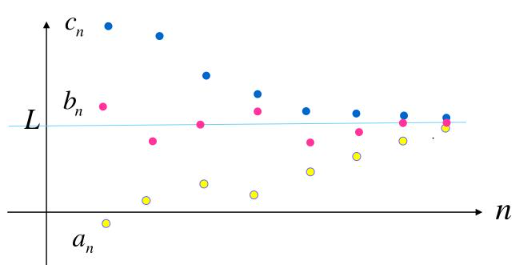
\includegraphics[width=0.7\linewidth]{squeeze.png}
    \end{figure}
\end{frame}

\begin{frame}{例}
    求
    \[
    \lim_{n\rightarrow\infty}\left(\frac{1}{n^2+n+1}+\frac{2}{n^2+n+2}+\cdots+\frac{n}{n^2+n+n}\right)
    \]
\end{frame}

\begin{frame}{反例}
    求
    \[
    \lim_{n\rightarrow\infty}\left(\frac{1}{n^2}+\frac{3}{n^2}+\cdots+\frac{2n+1}{n^2}\right)
    \]
\end{frame}

\begin{frame}{思路}
    \begin{itemize}
        \item 欲求极限的数列形如$\sum\limits_{i=1}^n\frac{f(i)}{g(i)}$,且不便通分
        \item 使用极限的定义:需要先知道极限的值
        \item 使用极限的四则运算法则:无穷个无穷小相加的值是不确定的
        \item 因此,考虑将$g(i)$放缩,将数列转化为容易计算的$\frac{1}{g(n)}\sum\limits_{i=1}^nf(i)$,
              再对其求极限.如此,可分别得到原数列极限的上限与下限.
        \item 上下限相同 $\Rightarrow$ 数列的极限=上限=下限
    \end{itemize}
\end{frame}

\begin{frame}{典例}
    求
    \[
    \lim_{n\rightarrow\infty}\left(\frac{1}{\sqrt{n^2-1}}-\frac{1}{\sqrt{n^2-2}}-\frac{1}{\sqrt{n^2-3}}-\cdots-\frac{1}{\sqrt{n^2-n}}\right)
    \]
\end{frame}

\subsection{区间套定理}

\begin{frame}{目录}
    \tableofcontents[currentsection]
\end{frame}

\begin{frame}{区间套定理}
    若$[a_{n+1},b_{n+1}]\subset[a_n,b_n],\ \forall n\in\mathbb{N}_+$,且有
    \[
    \lim_{n\rightarrow\infty}(b_n-a_n)=0,
    \]
    则存在唯一实数$\xi,\ \forall n\in\mathbb{N}_+$,有$a_n\le\xi\le b_n.$换言之,
    \[
    \xi\in\bigcap_{n=1}^\infty\ [a_n,b_n].
    \]
    \color{red}?
\end{frame}

\begin{frame}{思考}
    实数是如何定义的?

    \begin{itemize}
        \item 有理数:两个互质的整数$p,q$之商
        \item 无理数:\color{red}?
    \end{itemize}
\end{frame}

\begin{frame}{$\pi$的表示}
    \begin{itemize}
        \item 无理数都是“无限不循环小数”,例如$\pi,e,\sqrt2$.
        \item 尝试以小数形式表示$\pi$:
        \[
        \pi = 3.14159265358\ldots
        \]
        \item 只要这个小数只被写出来了有限项,那么它就是一个有理数.
        \item 只有当$\pi$所对应的小数的所有项,无限项都被写出,它才表示$\pi$.
    \end{itemize}
\end{frame}

\begin{frame}{尝试}
    \begin{itemize}
        \item 让我们尝试用有理数慢慢接近$\pi$.
        \item 只看整数部分,$\pi\in [3,4]$.
        \item 我们可以怎样让这个区间以一个稳定的方式不断缩小?
    \end{itemize}
\end{frame}

\begin{frame}{尝试}
    \begin{itemize}
        \item 让我们尝试用有理数慢慢接近$\pi$.
        \item 只看整数部分,$\pi\in [3,4]$.
        \item 二分,将$[3,4]$这个区间分成$[3,3.5],[3.5,4]$两个部分.
        \begin{itemize}
            \item 如果$\pi$落在左半边,则继续对左半边进行细分;右半边同理.
            \item 如果$\pi$同时落在两个区间内,那么它一定是两个区间所重合的那个数.这个数是一个有理数(为什么?)
        \end{itemize}
        \item 如此,第$n$次二分后得到的区间大小是$2^{-n}$.
        \item 当$n\rightarrow\infty ?$ 区间的大小趋近于$0$.
    \end{itemize}
\end{frame}

\begin{frame}{回到定义}
    若$[a_{n+1},b_{n+1}]\subset[a_n,b_n],\ \forall n\in\mathbb{N}_+$,且有
    \[
    \lim_{n\rightarrow\infty}(b_n-a_n)=0,
    \]
    则存在唯一实数$\xi,\ \forall n\in\mathbb{N}_+$,有$a_n\le\xi\le b_n.$
    \begin{itemize}
        \item $[a_{n+1},b_{n+1}]\subset[a_n,b_n],\ \forall n\in\mathbb{N}_+$:所取的区间长度不断缩小,且新区间总是前一个区间的子集.
        \item $\lim\limits_{n\rightarrow\infty}(b_n-a_n)=0$:区间长度最终趋近于$0$.
    \end{itemize}
    这样的\textbf{无穷个}区间套,共同定义着一个\textbf{实数}.
\end{frame}

\begin{frame}{证明}
    不难发现,对于每一次取子区间,总有:
    \[a_n\le a_{n+1} <\xi < b_{n+1} \le b_n\]
    \begin{itemize}
        \item $\{a_n\}$单调递增,且有上界$b_1$;
        \item $\{b_n\}$单调递减,且有下界$a_1$;
    \end{itemize}

    设$\lim\limits_{n\rightarrow\infty}a_n = A,\lim\limits_{n\rightarrow\infty}b_n = B$.
    $\quad\lim\limits_{n\rightarrow\infty}(b_n-a_n)=0 \Leftrightarrow A=B$
    
    夹逼定理$a_n\le\xi\le b_n$得证.$\square$
\end{frame}

% \begin{frame}{思考:$0.\dot{9}$和$1$相等吗?}

% \end{frame}

\begin{frame}{思考:$0.\dot{9}$和$1$相等吗?}
    \begin{itemize}
        \item 利用区间套定理
        \item $[a_1,b_1]=[0,1]$
        \item 此后不断将$a_n$增大至$0.\dot{9}$的小数点后$n$位
        \item $a_n=1-\frac{1}{10^n},b_n=1$
        \item 所逼近的数$0.\dot{9}=1$.
    \end{itemize}
\end{frame}

\begin{frame}{思考:$0.\dot{9}$和$1$相等吗?}
    直观理解:
    \begin{itemize}
        \item $0.\dot{9}$等价于$\lim\limits_{n\rightarrow\infty}0.\underbrace{999\ldots}_{n\text{个}9}=\lim\limits_{n\rightarrow\infty}(1-{\displaystyle\frac{1}{{10}^n}})=1$
    \end{itemize}
\end{frame}

\section{函数的极限}

\begin{frame}{思考}
    当我们讨论“极限”和“趋近于”时,我们在描述什么?
\end{frame}

\begin{frame}{引}
    从数列的极限中,我们知道:
    \begin{itemize}
        \item 对“无限趋近”、“极限”,可以使用$\epsilon-N$语言进行精确的表述.
        \item 含义:不论给定任意小的区间$(A-\epsilon,A+\epsilon)$,都能找到数列中的某一项$a_N$,使得
        这一项之后的所有项都落在这个区间内.当$\epsilon$足够小,$a_n$的值就几乎落在$A$这个点上.
        \item 核心是什么?
        \item 1.任意小的区间;\quad 2.能够使所有后续项落在该区间的$N$.
    \end{itemize}
\end{frame}

\begin{frame}{从$n\rightarrow+\infty$开始}
    \begin{enumerate}
        \item 任意小的区间:$\forall\epsilon>0,\dots,|f(x)-A|<\epsilon$
        \item 能使所有后续函数值都满足该条件的$X$:\\$\exists X\in D,\text{s.t.}\forall x>X,\dots$
    \end{enumerate} 
    连接起来:
    \[
    \forall\epsilon>0,\ \exists X\in D,\ \text{s.t.}\ \forall x>X,\ |f(x)-A|<\epsilon
    \]
\end{frame}

\begin{frame}{推广到$n\rightarrow-\infty$}
    \[
    +\infty:\quad\forall\epsilon>0,\ \exists X\in D,\ \text{s.t.}\ \forall x>X,\ |f(x)-A|<\epsilon
    \]

    \[
    -\infty:\quad\forall\epsilon>0,\ \exists X\in D,\ \text{s.t.}\ \forall x<X,\ |f(x)-A|<\epsilon
    \]
\end{frame}

\begin{frame}{推广到$n\rightarrow\infty$}
    \begin{itemize}
        \item 极限有唯一性.\\
        若$\displaystyle\lim_{x\rightarrow\infty}$存在,则极限应当同时存在于$+\infty$和$-\infty$处且相等.
        \item 为什么在数列极限中,只有$n\rightarrow\infty$而没有特别标明$+\infty$?
        \item 要求在正负无穷处取到同一极限值,那么值域应该是?
    \end{itemize}
\end{frame}

\begin{frame}{$\displaystyle\lim_{x\rightarrow\infty}f(x)$}
    设函数$f(x)$在$(-\infty,-a)\cup(a,+\infty)\ (a>0)$内有定义,若存在实数$A,\ \forall \epsilon>0,
    \ \exists X>0\color{red}{(X>a)},\ $使得当$|x|>X$时,
    \[
    |f(x)-A|<\epsilon,
    \]
    则称当$x$趋向于无穷时,函数$f(x)$的极限为$A$或$f(x)$收敛于$A$,记为
    \[
    \lim_{x\rightarrow\infty}f(x)=A\quad\text{或}\quad f(x)\rightarrow A\ (x\rightarrow\infty)\quad\text{或}\quad f(\infty)=A
    \]
\end{frame}

% \section{作业}

% \begin{frame}{HW2.T13.1}
%     设数集$E$有上界,证明:数集$-E:=\{x|-x\in E\}$有下界,且$\sup E = -\inf(-E)$.
% \end{frame}

% \begin{frame}{HW2.T13.2}
%     对非空数集$A,B$,定义其和为$A+B:=\{a+b|a\in A,\ b\in B\}.$
%     证明:若$A,B$皆有上界,则$A+B$亦有上界,且$\sup(A+B)=\sup A+\sup B.$
% \end{frame}

% \begin{frame}{HW2.T13.3}
%     若数列$a_n$满足$a_n<qa_{n-1}$,其中$a_n>0,0<q<1$,试用定义证明$\lim\limits_{n\rightarrow\infty}a_n=0$.
% \end{frame}

% \begin{frame}{HW2.T13.4}
%     设有数列$\{a_n\}$和$\{b_n\}$,如果$\lim\limits_{n\rightarrow\infty}\frac{a_n}{b_n}=a(a\ne0)$且$\lim\limits_{n\rightarrow\infty}a_n=0$,
%     证明$\lim\limits_{n\rightarrow\infty}b_n=0.$
% \end{frame}

% \section*{}
% \begin{frame}{反馈问卷}
%     \begin{figure}[H]
%         \centering
%         
\includegraphics[width=0.5\linewidth]{qrcode.png}
%     \end{figure}
% \end{frame}
% -------------------------------------------------------
% \section*{}
% \begin{frame}
% \vspace{25pt}
% \[
% \text{\Huge Office Hour}
% \]
% \end{frame}

\end{document}